\documentclass[12pt]{article}
\usepackage{float}
\usepackage[german,english]{babel}
\usepackage{epsf}
\usepackage{latexsym}
\usepackage{epsfig}
\usepackage {amssymb}
\usepackage {amsmath}
\usepackage{color}
\setlength{\parindent}{0 cm}
\usepackage{setspace}
\linespread{0.95}

\setlength{\textwidth}{15cm} \setlength{\textheight}{22cm}
\topmargin-1.5cm \evensidemargin0.5cm \oddsidemargin0.5cm

%\headheight0cm \headsep0cm \topskip0cm
\parindent3ex \parskip1.5ex plus 0.5ex minus 0.3ex

\usepackage{rotating}

\usepackage[longnamesfirst]{natbib}
\bibpunct{(}{)}{;}{a}{,}{,}
\renewcommand{\cite}{\citep}
\newcommand{\biblist}{
\bibliographystyle{apalike}
\bibliography{Literature}
}

\setlength{\bibsep}{0cm}

\usepackage{epsfig}
\def\beqn{\begin{eqnarray*}}
\def\eeqn{\end{eqnarray*}}
\def\beq{\begin{eqnarray}}
\def\eeq{\end{eqnarray}}
\def\bm#1{\mbox{\boldmath{$#1$}}}

\def\sumkKn{\sum_{k=1}^{K_n}}
\def\sumin{\sum_{i=1}^n}
\def\eps{\varepsilon}
\def\t{{\rm t}}
\def\var{\mbox{var}}
\def\cov{\mbox{cov}}
\newcommand{\leftsup}[2]{{\vphantom{#2}}_{#1}{#2}}

%\def\myfootnote[#1]#2{\begingroup%
%\def\thefootnote{\fnsymbol{footnote}}\footnote[#1]{#2}\endgroup}

\newtheorem{lemma}{Lemma}
\newtheorem{theorem}{Theorem}


\makeatother
\makeatletter
\renewcommand{\@fnsymbol}[1]{\@arabic{#1}}
\makeatother
\title{A statistical view on ``Predicting reaction performance in C--N cross-coupling using machine learning''}

\author{Tatyana Krivobokova\footnote{Department of Statistics and Operations Research,
Oskar-Morgenstern-Platz 1, 1090 Wien}\\{Universit\"at Wien}
\and Boris Maryasin\footnote{Department of Organic Chemistry, W\"ahringer Stra{\ss}e 38, 1090 Wien}\\{Universit\"at Wien}
\and Gianluca Finocchio$^1$\\{Universit\"at Wien}
} 


\begin{document}

\baselineskip=25pt

\maketitle

\begin{abstract}

\baselineskip=15pt \noindent The data collected in \citet{Ahneman2018} are revisited and rigorously analysed. It is shown that the matrix of chemical descriptors is up to a linear transformation equivalent to a dummy coded matrix that reflects the design of the underlined experiment. Moreover, this matrix is ill-conditioned and therefore hinders interpretability of any estimated models. It is argued that the reaction yield should be modelled as a continuous Bernoulli random variable. Finally, a four way ANOVA with single replicates following a continuous Bernoulli distribution is fitted to the data under the assumption of sparsity of the parameters. It is found that four levels interactions are not significant and most significant parameters in a three levels interaction model are identified and interpreted.  

%{\textit{Key words and phrases.}} Continuous Bernoulli distribution, designed experiment, generalised partial least squares
\end{abstract}

%%%%%%%%%%%%%%%%%%%%%%%%%%%%%%%%%%%%%%%%%%%%%%%%%%%%%%%%%%%%%%%%%%%%%%
%%%%%%%%%%%%%%%%%%%%%%%%%%%%%%%%%%%%%%%%%%%%%%%%%%%%%%%%%%%%%%%%%%%%%%
%%%%%%%%%%%%%%%%%%%%%%%%%%%%%%%%%%%%%%%%%%%%%%%%%%%%%%%%%%%%%%%%%%%%%%

\baselineskip=20pt
\section{Introduction}
{\color{red} @ Boris: it seems that in Science there are no sections per se; I am not sure how we should write it for now; in any case, we need some kind of introduction, saying about data and machine learning in chemistry, about the Ahnemann paper, the comment on it with critics and may be more examples of similar papers?} 
\label{sec:intro}
\doublespacing
\linespread{1.2}


\section{Data and statistical model}
\label{sec:model}
{\color{red} @Boris: please describe the reaction, data generation process, what is special, give them credit for impressive data set etc}\\
Hence, the data at hand are the yield values (between $0$ and $100$) observed for $3960$ combinations of four factors. In the following we discuss that the direct application of machine learning techniques, without taking into account the specific properties and structures of the data, may lead to suboptimal estimation and inference, as well as to improper interpretation of the results. Subsequently, we consider properties of the response variable and structures in the covariates matrix. 
\subsection{Response variable modelling}
\label{subsec:response}
In a statistical model the response variable, which is in our case the yield of the reaction, is treated as a random variable. From the histogram of the yield, shown on the left plot of Figure \ref{Fig1}, as well as in the Suplementary Material to \citet{Ahneman2018} (Figure S7), it is obvious, that this random variable has a bounded support (can not take values outside $[0,100]$ interval) and its distribution is right skewed (more reactions have a lower yield). Modelling the yield as a symmetric random variable with unbounded support, e.g., as a normally distributed random variable, would lead to a prediction, that may end up outside the possible range of values in $[0,100]$, as well as to a wrong inference. 
Indeed, this is observed in the middle plot of Figure \ref{Fig1}, which is obtained as follows. First, a standard linear model is fitted on a training set, as if the yield has an unbounded support, and then the prediction is made on the test set. The squared Pearson correlation and the root mean squared error between the true yield on the test set and it's prediction from a linear model on the same set correspond to those reported in \citet{Ahneman2018}. As in the original publication, the predicted values of the yield take impossible negative values (up to minus $50$) and do not show a clear linear relationship to the observed yield values. 
\begin{figure}[t]
	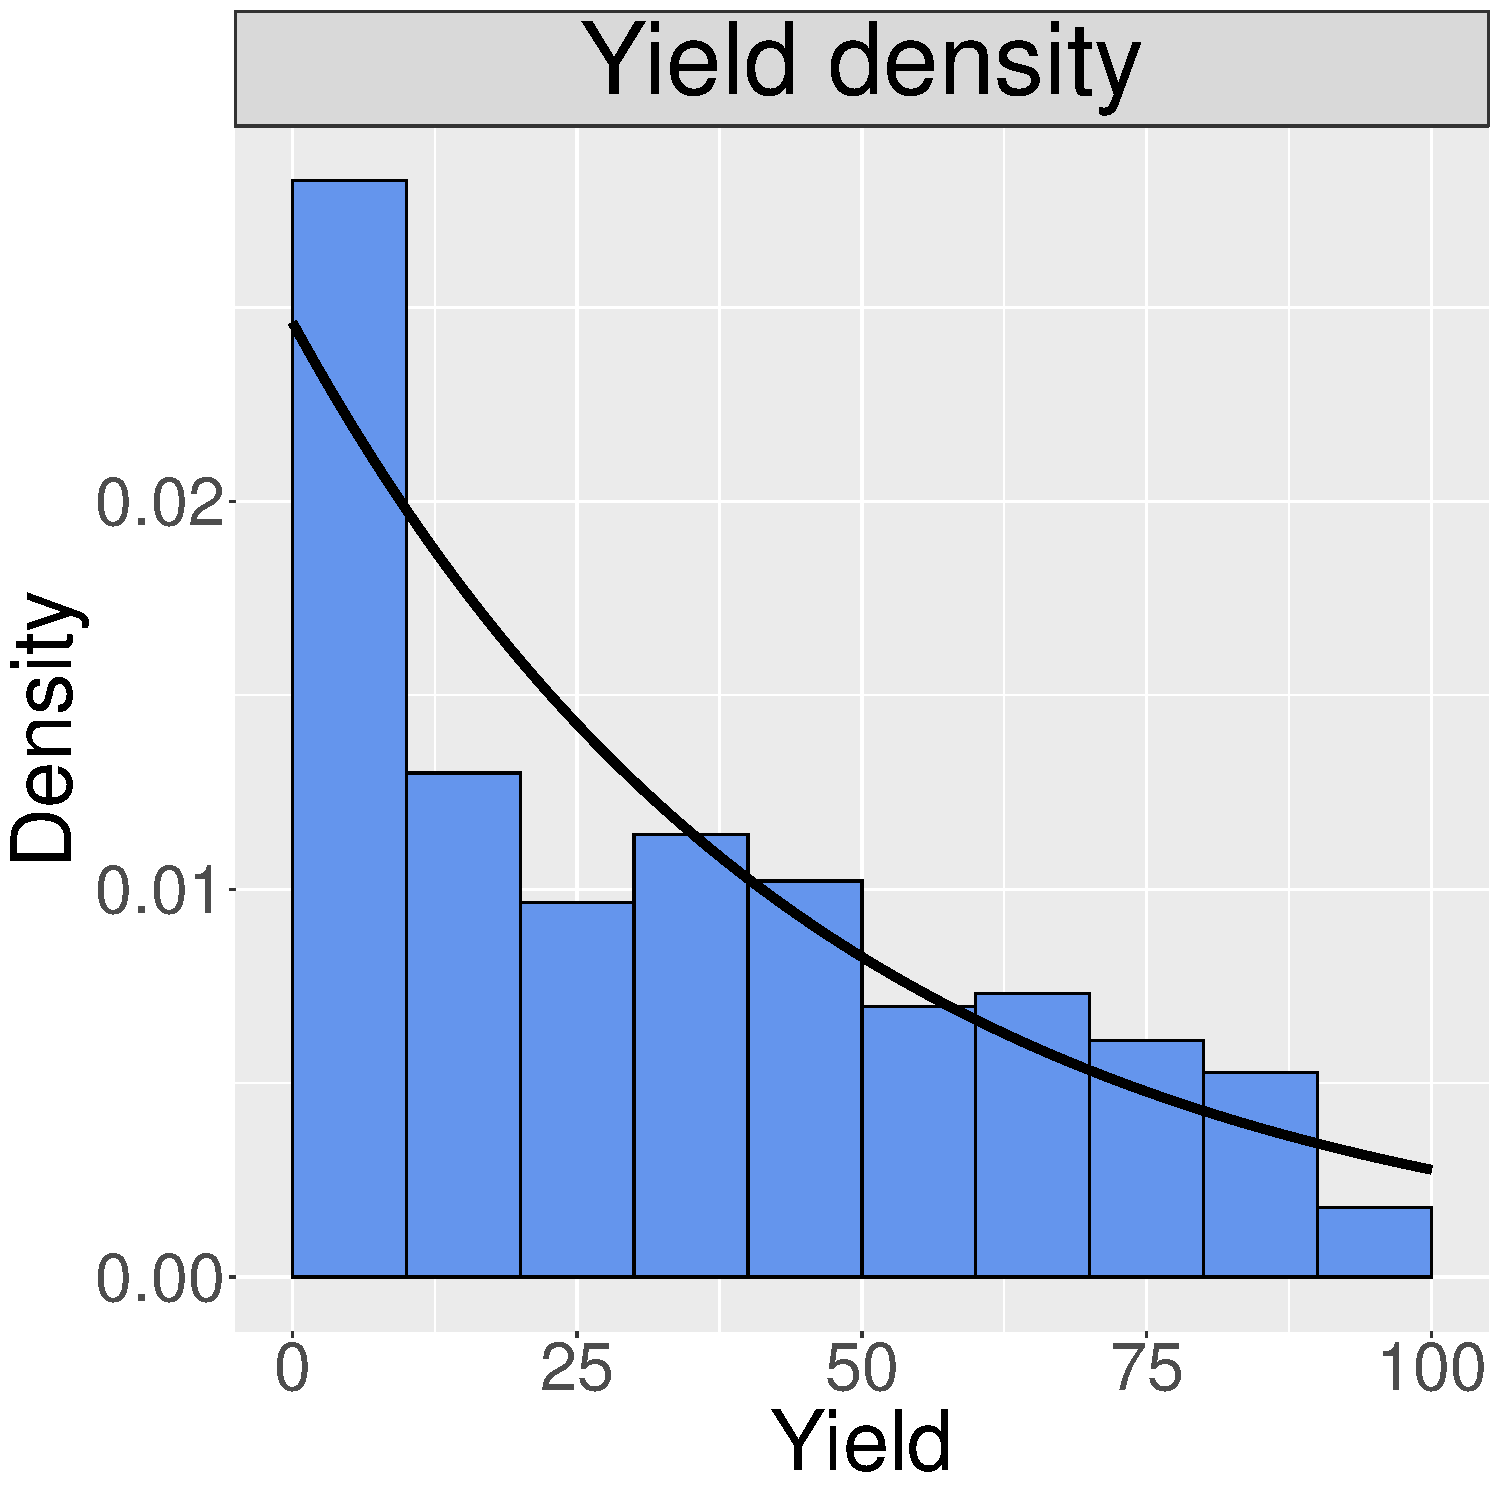
\includegraphics[width=0.33\textwidth]{Plots/yield_hist.pdf}
	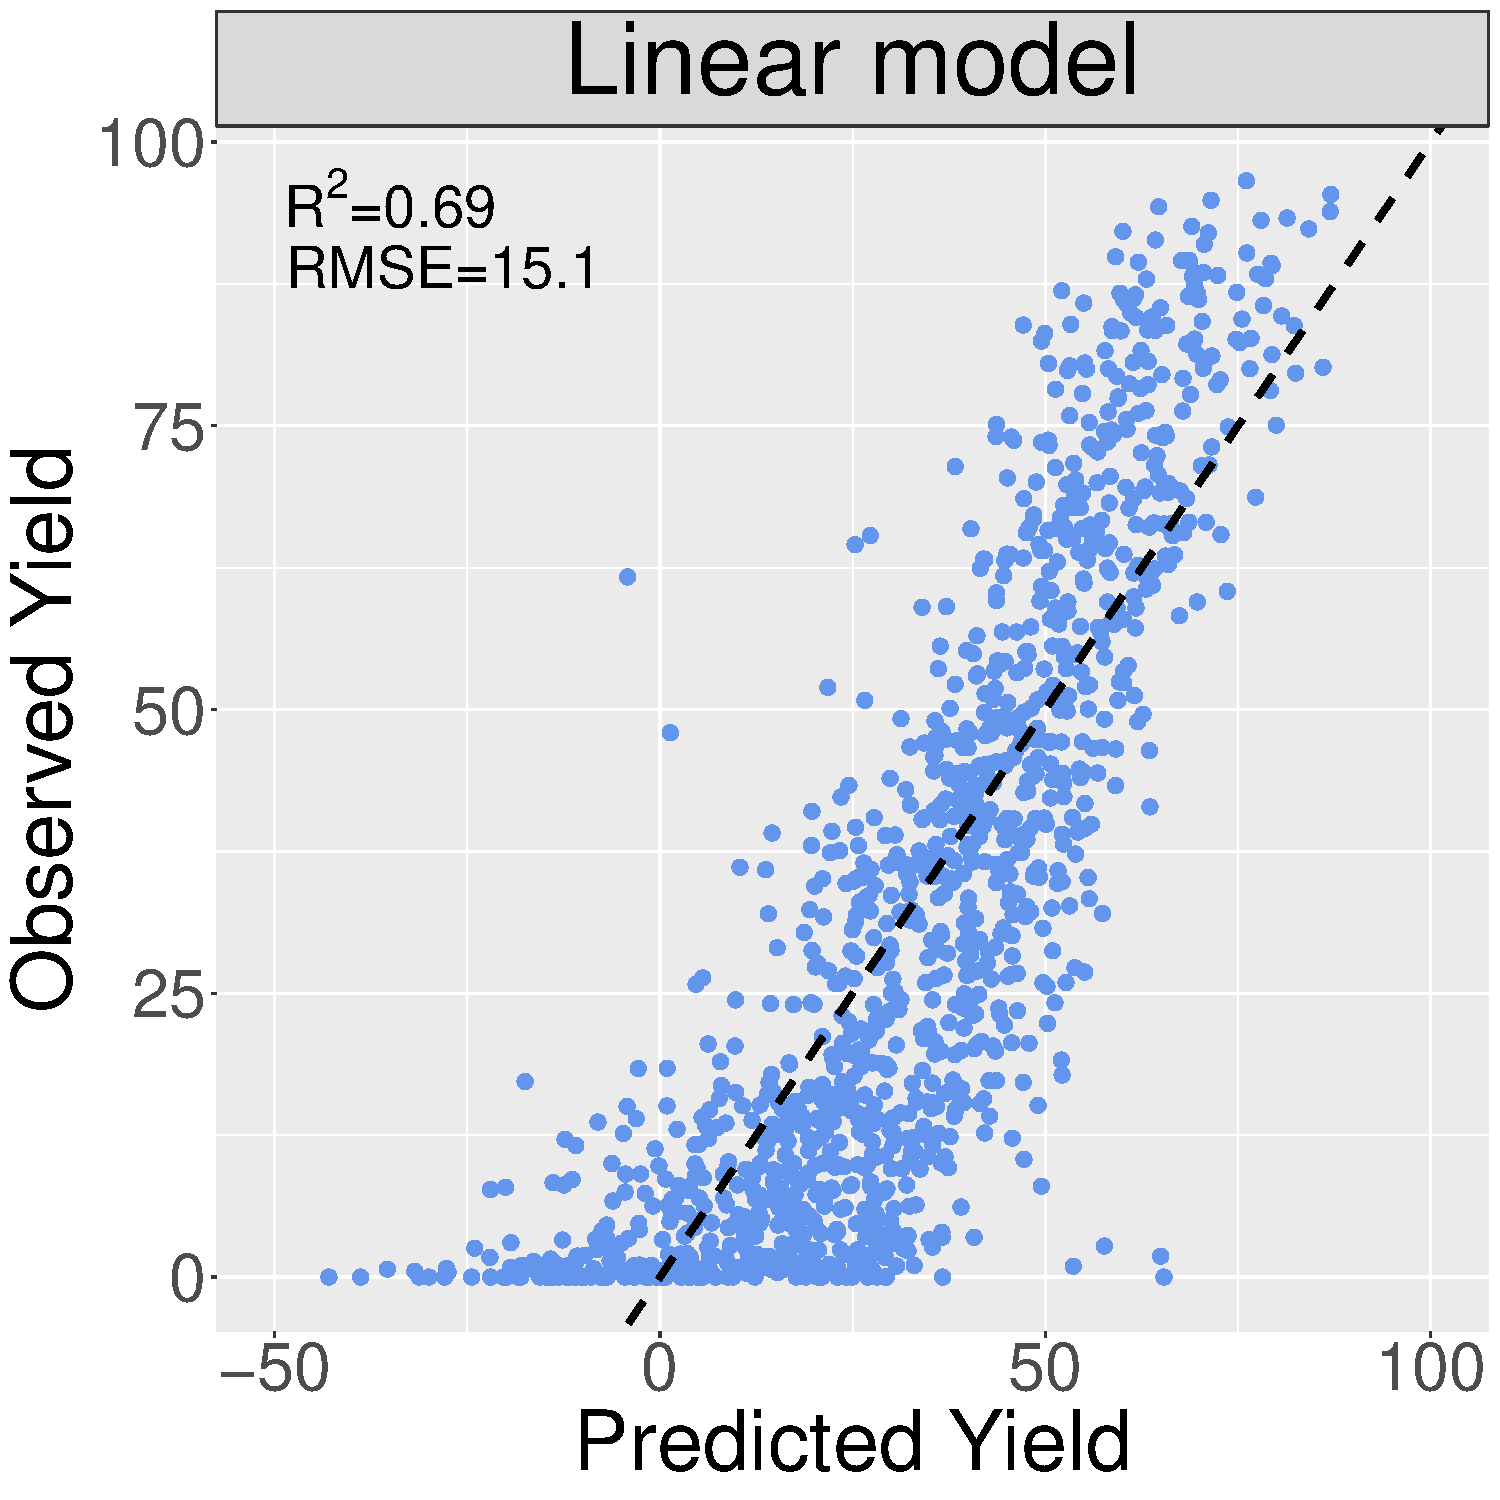
\includegraphics[width=0.33\textwidth]{Plots/linear_model.pdf}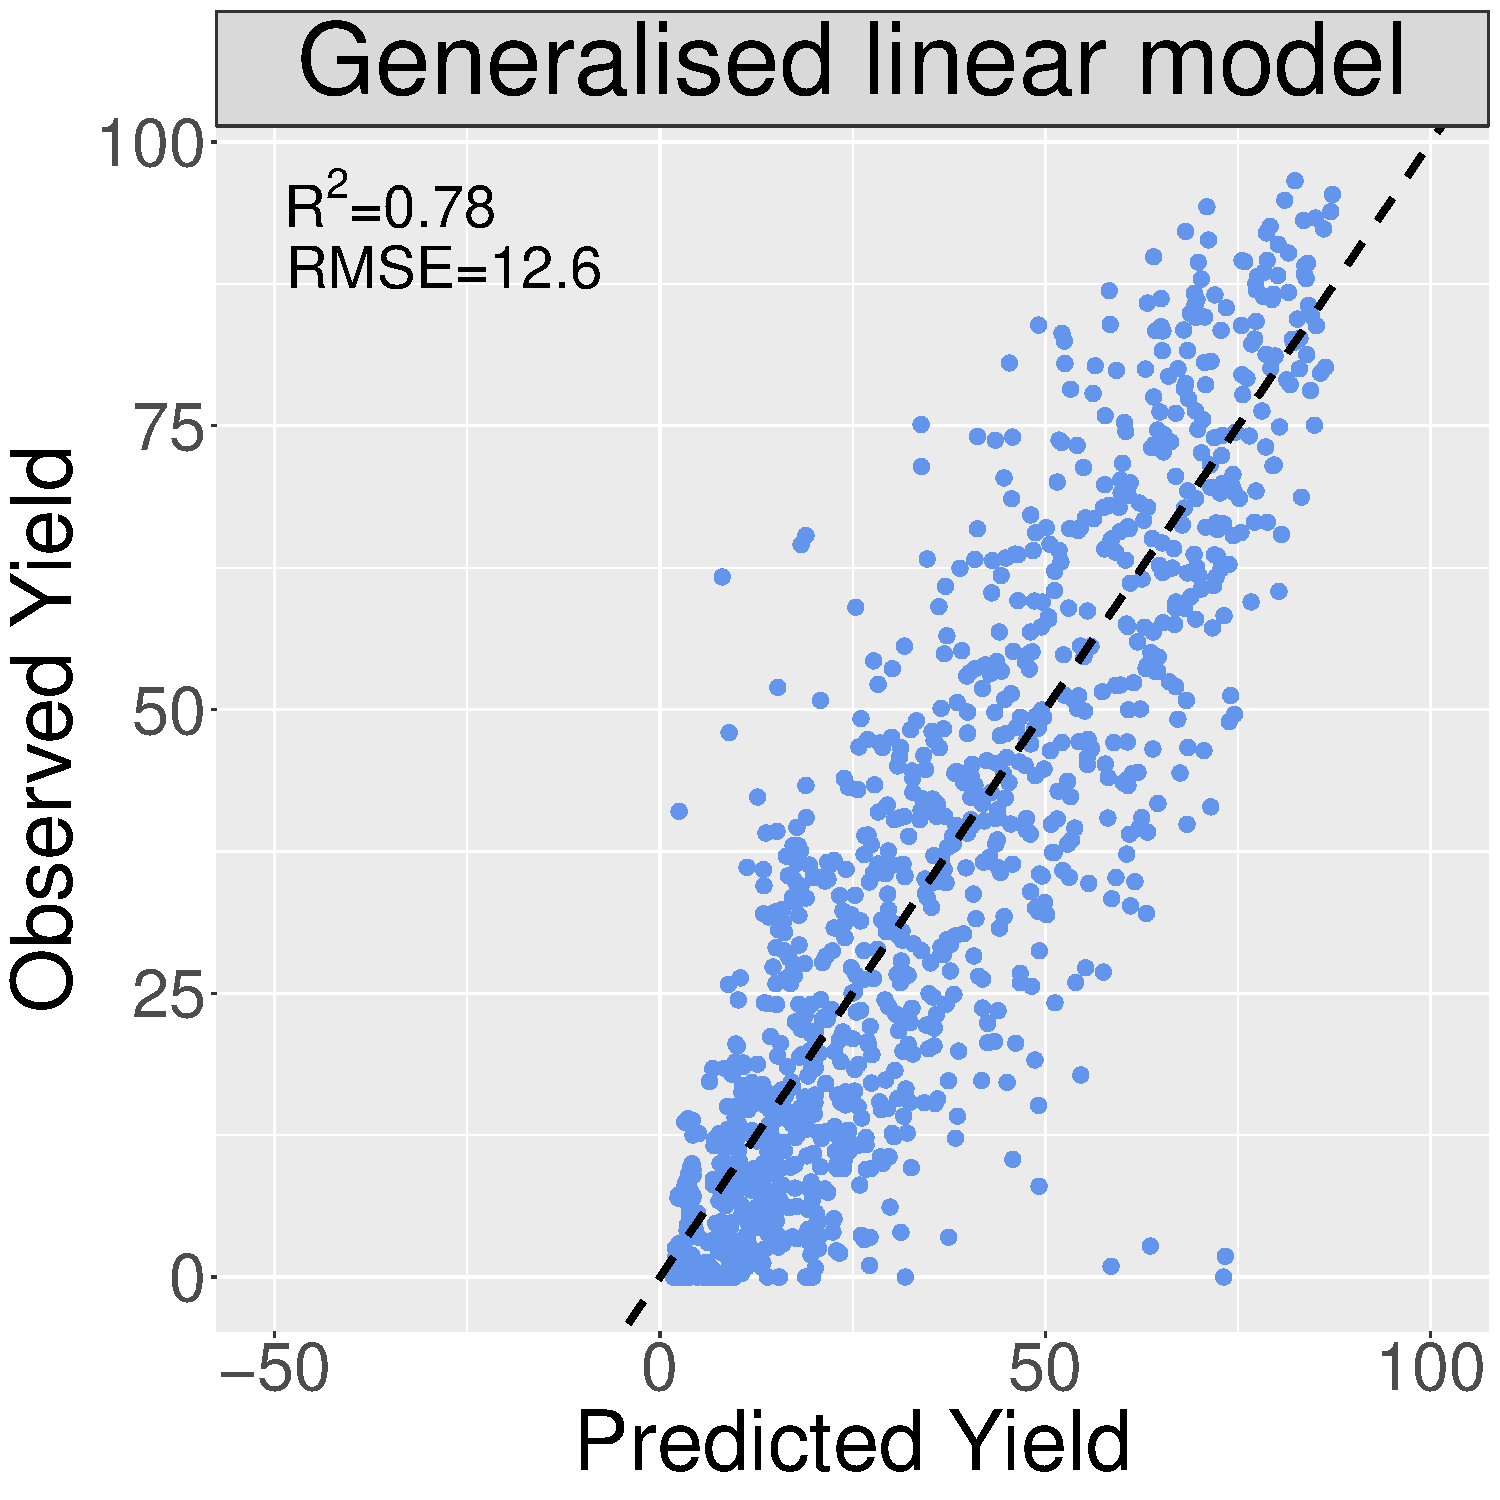
\includegraphics[width=0.33\textwidth]{Plots/cb_model.pdf}
	\caption{Yield histogram with the density of a continuous Bernoulli distribution (left); Yield prediction with a linear model (middle); Yield prediction with a generalised linear model (right)}
	\label{Fig1}
\end{figure}
Obviously, inference about regression coefficients based on the assumption of normality of the yield would also be flawed. \\
Instead, it seems reasonable to model the yield by a continuous Bernoulli distribution. The density of the continuous Bernoulli distribution is given by
\beqn
f(y;p)=\begin{cases}
	\frac{\log\{(1-p)/p\}}{1-2p}p^y(1-p)^{1-y},&p\in(0,1), \;p\neq 0.5\\
	2\,p^y(1-p)^{1-y},&p=0.5,
\end{cases}
\eeqn 
for $y\in[0,1]$ and parameter $p$ being a success probability. A maximum likelihood estimator for $p$ based on the yield data resulted in $\hat{p}=0.1$, with the corresponding density function shown in the left plot of Figure \ref{Fig1} as a bold line. Since continuous Bernoulli distribution is a member of the natural exponential family, this allows to employ the well-established Generalised Linear Model (GLM) framework for estimation and inference, details are provided in the Supplementary material. 
The resulting prediction is shown in the right plot of Figure \ref{Fig1}. Obviously, all predicted yield values are now inside the $[0,100]$ interval and show a much better linear relationship to the observed yield. Moreover, the root mean squared error has improved from $15.1$ to $12.6$, while the squared Pearson correlation increased from $0.69$ to $0.78$. \\
In general, (generalised) linear model framework has various practical advantages over non-parametric methods, including fast estimation, immediate inference about the regression coefficients, easy prediction and straightforward interpretation. However, in practice, both inference and  interpretability of a (generalised) linear model depend heavily on the properties of the matrix of covariates, which we discuss next. 
\subsection{Structures in covariates}
\label{subsec:covariates}
In the original work of \citet{Ahneman2018} the matrix of covariates consists of $120$ variables. However, an eigendecomposition of this matrix immediately detects that only $39$ columns of that matrix are linearly independent. Hence, the columns that are perfectly linearly dependent should be removed before the analysis. In the remaining full-rank matrix with $39$ columns, it is advisable to look at the corresponding condition number. If a full-rank matrix of covariates is ill-conditioned, then the corresponding regression coefficient estimators are prone to very large numerical errors and are practically not interpretable. Note, however, that the prediction with such regression coefficients still might be reasonable: with an ill-conditioned matrix of covariates one can get nearly same predictions with different sets of regression coefficients. It turns out, that the condition number of the matrix at hand is of order $10^{7}$, so that the analysis done in \citet{Ahneman2018}, while delivering a reasonable prediction, should have interpretability problems. A high condition number indicates that the matrix of covariates contains highly correlated columns, which is indeed the case for the matrix of chemical descriptors, as can easily be checked. Random forest algorithms are especially affected by highly correlated covariates. It is well-known that the correlated covariates can improve the cross-validated performance of the random forest algorithm, but lead to improper interpretation, see e.g., \citet{10.1093/bioinformatics/btr300} or \citet{Gregorutti2017}. In fact, \citet{Chuang2018} already discussed that the predictors, identified by \citet{Ahneman2018} from a random forest fit as most influential for the yield, seem to be misleading. \\
In the same work \citet{Chuang2018} also hypothecise that the analysis performed in \citet{Ahneman2018} ``exploits patters within the underlying experimental design, instead of learning solely from meaningful chemical features''. In the following we show that this hypothesis indeed holds true. \\
Matrix of $120$ covariates given in \citet{Ahneman2018} contains $19$ descriptors of {\color{blue} additive}, $27$ descriptors of {\color{blue} aryl halide}, $10$ descriptors of {\color{blue} base} and $64$ descriptors of {\color{blue} ligand}. {\color{red}@Boris: I am not sure how we should address these factors (descriptors), I wrote them everywhere in blue, so that one can see where these should be updated for more suitable notions} Since the data are collected in a designed experiment as described above, each descriptor of {\color{blue} additive, aryl halide, base and ligand} has only $22$, $15$, $3$ and $4$ distinct values, respectively. In particular, the rank of the sub-matrix, that contains $64$ descriptors of {\color{blue} ligand} equals to $4$, since there are only $4$ distinct rows in that sub-matrix. In the same manner, the rank of the sub-matrix that contains $10$ descriptors of {\color{blue} base} equals to $3$ and the rank of the sub-matrix with $27$ descriptors of {\color{blue} aryl halide} is $15$. Since there are only $19$ descriptors for {\color{blue} additive} with $22$ possible values, the rank of that sub-matrix is $19$. Removing all linear dependent covariates results in a matrix with $39$ columns. If there were $22$ descriptors for {\color{blue} additive} (one can add three random descriptors), the rank of the whole matrix would be $41$ and this matrix can be uniquely transformed to obtain a matrix with dummy (or one-hot) coding, since both matrices are of full rank and span the space of the same dimension, see Supplementary materials for the exact derivations. In particular, this means that the values of chemical descriptors carry no meaningful information and one can code only absence or presence of a certain feature. Therefore, in practice there is no need to use the matrix of chemical descriptors, which is ill-conditioned and lacks three columns; one should directly build a dummy matrix that corresponds to the given experimental design. \\
Hence, the linear regression model estimated in \citet{Ahneman2018} (its prediction on the test set is shown in the middle plot of Figure \ref{Fig1}) is (nearly) equivalent to an ANOVA model with four factors without interactions and with $30\%$ of observations randomly missed (moved to the test set):
$$
\mbox{yield}_{ijkl}=\mu_0+\alpha_i+\beta_j+\gamma_k+\delta_l+\epsilon_{ijkl},
$$
where $\mu_0$ is an overall mean, $\alpha_i$, $i=1,\ldots,22$ is the deviation of $i$-th level of the factor {\color{blue} additive} from $\mu_0$, $\beta_j$, $j=1,\ldots,15$ is the deviation of $j$-th level of the factor {\color{blue} aryl halide} from $\mu_0$, $\gamma_k$, $k=1,2,3,4$ is the deviation of $k$-th level of the factor {\color{blue} ligand} from $\mu_0$ and $\delta_l$, $l=1,2,3$ is the deviation of $l$-th level of the factor {\color{blue} base} from $\mu_0$. For identifiability, it is assumed that $\sum_i\alpha_i=\sum_j\beta_j=\sum_k\gamma_k=\sum_l\delta_l=0$. Apparently, this ANOVA model can be written as a linear regression, where the matrix of covariates is represented with a dummy coding, see Supplementary materials for details. Note, that this representation of the model leads to the covariates matrix with a much lower condition number (around $25$). \\
%All together, the matrix of chemical descriptors is up to a linear transformation (nearly) equivalent to a dummy coded matrix of the given designed experiment, but it lacks three columns and is ill-conditioned, so that it should not be used in practice.  \\
Hence, the hypothesis of \citet{Chuang2018} holds true and \citet{Ahneman2018} essentially applied several machine learning algorithms to estimate the yield based on an ANOVA model with missing values (which constitute the training set) and predict those missing values. It is important to stress that the analysis of \citet{Ahneman2018} can not be used for interpretation and generalisation to unseen chemical descriptors values. In a designed experiment with a multi-factor ANOVA model the focus is typically on identification of significant factor levels and their combinations, which has not been done in \citet{Ahneman2018}. In the next section we discuss an appropriate statistical model and the corresponding analysis for the data generated by \citet{Ahneman2018}.
\subsection{Four factor generalised ANOVA with single replicates}
In the previous sections we discussed that the data collected by \citet{Ahneman2018} have the following features: the response variable contains the values of reactions yields that follow a continuous Bernoulli distribution. Moreover, the values of that response variable have been measured in a designed experiment: there are four factors ({\color{blue} additive, aryl halide, ligand and base}) and under each combination of the factor levels there is a single observation available. Hence, the corresponding generalised ANOVA model can be written as follows
\beq
\label{eq:anovamodel}
g\left\{\mbox{E}(\mbox{yield}_{ijkl})\right\}&=&\mu_0+\alpha_i+\beta_j+\gamma_k+\delta_l+(\alpha\beta)_{ij}+(\alpha\gamma)_{ik}+(\alpha\delta)_{il}+(\beta\gamma)_{jk}\nonumber \\
&+&(\beta\delta)_{jl}+(\gamma\delta)_{kl}+(\alpha\beta\gamma)_{ijk}+(\alpha\beta\delta)_{ijl}+(\beta\gamma\delta)_{jkl}\\
&+&(\alpha\gamma\delta)_{ikl}+(\alpha\beta\gamma\delta)_{ijkl},\nonumber
\eeq
where all the parameters are as defined before with extra terms representing interaction effects between corresponding levels and $g(\cdot)$ is a canonical link function for a continuous Bernoulli distribution, see Supplementary materials. Since there is only one yield replication per each combination of four factor levels, there is only one observation for each parameter estimator available and a regular maximum likelihood estimator for all the parameters would be too variable. However, it is reasonable to assume that a big share of $3960$ parameters in this large model is not significant. This is supported by the observation that estimators for the model with interactions of two factors already become numerically unstable due to many parameters being estimated close to zero. Hence, there is a need for some sort of regularisation.\\
In a similar context for a two-way ANOVA with single replicates \citet{GRIFFIN2019181} assumed that the interaction coefficients are sparse (that is, most of them are close to zero) and suggested to employ a lasso penalisation for the parameters, using Bayesian framework. This approach can not be directly employed for the data at hand, since the yield is not normally distributed and there are four factors in the model. Instead, we suggest a new approach based on the partial least squares (PLS) algorithm, which enjoys a wide applicability and popularity in chemometrics. Originally, this algorithm has been suggested by \citet{Wold66} in the usual regression context. Extension of PLS to the responses from the exponential family is not trivial and has been recently addressed in {\color{red}@Gianluca: may be we'll be able to put something to arxiv later in September; also please add some advantages of PLS}. \\
First, we estimated the model (\ref{eq:anovamodel}) with all possible interaction effects. It turned out, that none of the four levels interaction terms seemed to be significant. Next, a model without four levels interactions has been estimated. This resulted in an estimator with nearly the same value of the log-likelihood, so that the analysis of the deviance confirms that four levels interactions are not significant. Thereby, estimators for several three levels interactions were very large. Trying to reduce the model further, that is, omitting all three levels interactions, lead to a loss in the log-likelihood. We have to note that a rigorous statistical inference in such models is a very challenging task and will be addressed in a separate work. We conclude that four levels interactions are not significant for these data, but several three levels interaction bring significant deviations from the overall mean $\mu_0$. \\
Since the chemical descriptors itself carry no meaningful information, but only their levels, we restrict ourselves to {\color{blue} additive C3 NMR shift, aryl halide C2 electrostatic charge, base dipole moment and ligand C11 electrostatic charge}. The largest positive effects on the yield have a combination of {\color{blue} additive 152.98} and {\color{blue} aryl halide 0.392}. The second largest positive effect on the yield has the combination of {\color{blue} additive 143.12} and {\color{blue} base 1.126}. The two largest negative effects are by {\color{blue} aryl halide 0.392} and {\color{blue} aryl halide 0.040} along. \\
{\color{red} @Boris: we have to discuss how to describe all these effects and how to interpret them; here is the table}
\begin{verbatim}
	                         intercept 				-6.99658737516461
                  aryl_halide last 				 7.05891363753285
          aryl_halide 11:ligand 	4  			-7.7384871004874
                         additive 16 					-8.14417962647228
                      aryl_halide 2 					 8.57032851178768
 additive 18:aryl_halide 9:base 2  		9.14811873197853
 additive 18:aryl_halide 9:base 3  		10.0200286097766
                additive 10:base 2  			11.1917082030815
                additive 10:base 3 			-11.8154611716124
            additive 15:base last 			-12.6230891563856
                        additive 10 				-14.0296781441994
                     aryl_halide 11 			-15.4202953497052
         additive 18:aryl_halide 9  	   	23.3251100360785
                      aryl_halide 9				 -28.8683600594159
\end{verbatim}

\label{subsec:stat_model}
\section{Discussion}
{\color{red} Here I would probably add on the random forest model performance in the original paper and its possible application (imputation), not to kill their paper completely and stress that we give a different and useful analysis}
\label{sec:discussion}


\section*{Acknowledgements}
TK is grateful to Efstathia Bura for helpful discussions.
%%%%%%%%%%%%%%%%%%%%%%%%%%%%%%%%%%%%%%%%%%%%%%%%%%%%%%%%%%%%%%%%
%%%%%%%%%%%%%%%%%%%%%%%%%%%%%%%%%%%%%%%%%%%%%%%%%%%%%%%%%%%%%%%%
%%%%%%%%%%%%%%%%%%%%%%%%%%%%%%%%%%%%%%%%%%%%%%%%%%%%%%%%%%%%%%%%

\begin{appendix}
\label{appendix}
\end{appendix}

\biblist

\end{document}
